\subsection{Rejection Regions and Power}
\label{subsec:rejection-region-and-power}

\begin{figure}[H]
  \centering
  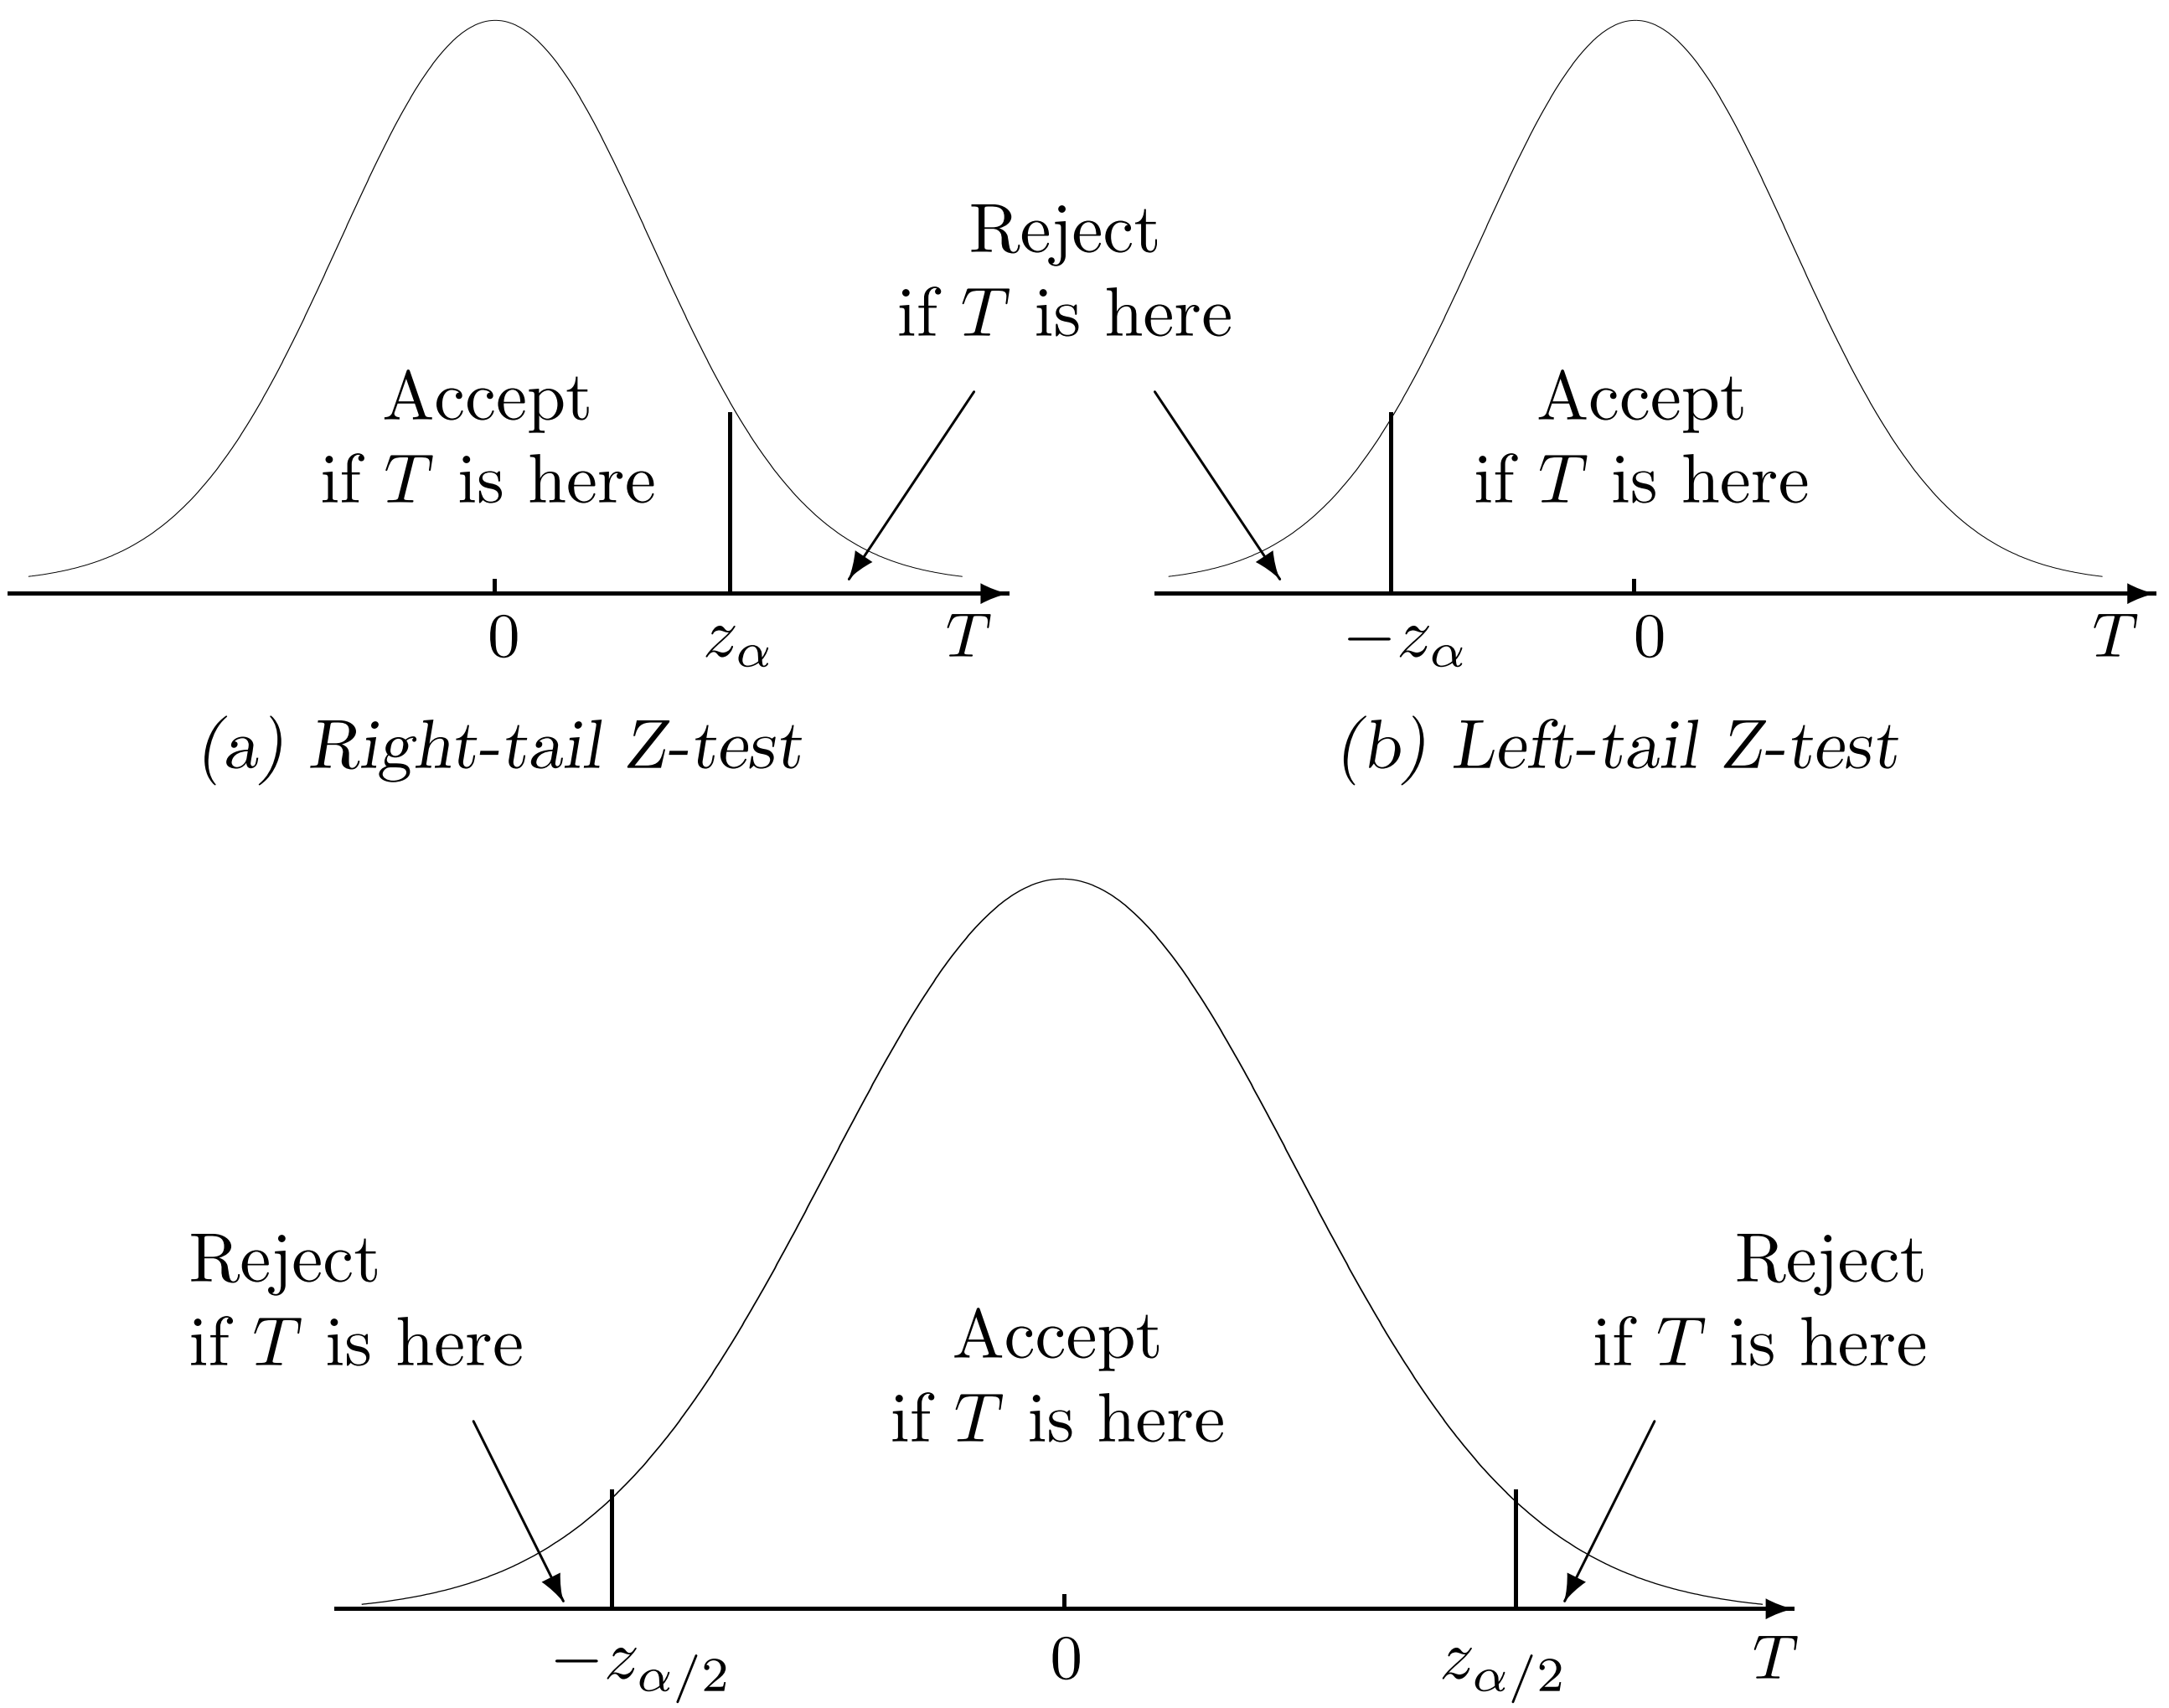
\includegraphics[width=\linewidth]{img/fig-9.7.png}
  \caption{\textit{Acceptance and rejection regions for a $Z$-test with (a) a one-sided right-tail alternative; (b) a one-sided left-tail alternative; (c) a two-sided alternative.}}
  \label{fig:9.7}
\end{figure}

\begin{itemize}[leftmargin=.6cm]
  \item For a \textbf{right-tail alternative}, the rejection region $\mathcal{R}$ should consist of large values of $T$ . Choose $\mathcal{R}$ on the right, $\mathcal{A}$ on the left (Figure 6a).
  \item For a \textbf{left-tail alternative}, the rejection region $\mathcal{R}$ should consist of small values of $T$ . Choose $\mathcal{R}$ on the left, $\mathcal{A}$ on the right (Figure 6b).
  \item For a \textbf{two-sided alternative}, the rejection region $\mathcal{R}$ should consist of very small and very large values of $T$ . Let $\mathcal{R}$ consist of two extreme regions, while $\mathcal{A}$ covers the middle (Figure 6c).
\end{itemize}
